\section{Simulator}
\label{chap:4}

  
This section presents the structure of the simulator and a brief tutorial ``\textbf{How to use my project}". The simulator was written in Elixir 1.3. Elixir is a dynamic functional programming language designed for building fault-tolerant, scalable and maintainable application. Elixir is based on Erlang virtual machine Beam, widely used for building fault-tolerant distributed systems. The project includes a topology generator written in python. The topology generator is an open-source implementation under MIT license that was customised for this project. The original code can be found here \url{https://github.com/tcoyze/stochastic-blockmodel}. The repository of the full project is in \url{https://github.com/mtileria/SymmetryBreaking} including the modified topology generator. The graphs were plotted using the language R.



\subsection{Simulator Structure}

The simulator is based on the Actor model for concurrent systems. In Elixir, all programs run inside an isolated lightweight process that only communicates with other processes via messages passing. Regarding the \textit{MIS} algorithm implementation, there is a mapping from the graph to the processes. Every vertex of the graph is associated with an elixir process that runs the same distributed algorithm. The communication channel among processes represents the edges of the graph. 

\textbf{Mix} is an Elixir tool for creating, compiling and testing applications. This tool was used to create the project template. In the simulator directory, the sub-directory \textbf{config} is created by default and contain the project configurations.  The implementation of the algorithm are in the \textbf{lib} directory, which has three sub-directories (\textbf{global}, \textbf{alpha} and \textbf{beta}), one for each synchronisation technique.

The complete project structure is presented below. The two main directories are ``\textbf{generator}" and ``\textbf{simulator}". The code related to the synchronous simulation and \textit{MIS} are in the simulator directory while the topology generator is in the generator directory. 


\begin{verbatim}
SymmetryBreaking/
|
|--generator
|  |-- graph
|  |-- topologies
|  main.py
|--simulator
|  |-- config
|  |-- files
|  |-- lib
|      |-- beta
|           |-- Beta.ex
|           |-- sync_mis_beta.ex
|           |-- b_controller.ex
|      |-- alpha
|           |-- alpha.ex
|           |-- sync_mis_alpha.ex
|           |-- a_controller.ex
|      |-- global
|           |-- g_mis.ex
|           |-- g_controller.ex
|  |--results
|  |--test
\end{verbatim}

\subsection{MIS with Global Synchronizer}
 
The implementation of the \textit{MIS} algorithm with the global synchronizer is in the directory \textbf{simulator/lib/global}. The \textbf{MIS} algorithm is in the file \textbf{g\_mis.ex} and file \textbf{g\_controller.ex} contains the module \textbf{GlobalSync} which handle the start and finish of the simulation, also the synchronisation mechanism and store the metrics.

In the \textbf{GlobalSync} module, the function \textit{start\_nodes n} is the start point of the simulation, where \textbf{n} is the number of processes to be spawned. This function is in charge of spawn the processes that are going to run the \textit{MIS} algorithm, henceforth active processes. The first task of this function is to spawn the master process, which is the one that it is going to indicate actives processes when to start the algorithm.  Besides that, the master process controls when a new round starts and receives the output of the processes at the end of the algorithm.

Actives processes are spawned according to the information in the files  \textbf{N\_nodes.txt} and \textbf{N\_edges.txt}. These files are generated previously with the topology generator. The simulator read the topology information from the files and creates the network.  

For the global simulation, the implementation is described with details in this section. For the Alpha and Beta implementation, only the differences with the global synchronisation are listed. The  \textit{start\_nodes n} function is illustrated in the code \ref{code:start}.


\begin{lstlisting}[frame=single, columns=fullflexible, mathescape=true, caption= start\_nodes function, label = code:start]


def start_nodes (n) do
  master_id = spawn(GlobalSync,
  :run_master,[GlobalSync.init_master(n)])
  case :global.register_name(:master,master_id) do
    :yes -> master_id
    :no -> :error
  end

  stream = File.stream!("N_nodes.txt")
  p_names = String.split(List.first(Enum.take stream,1))
  p_ids = for name <- p_names do
    pid = spawn(MIS,:run, [MIS.init_state(name, master_id)])
    case :global.register_name(name,pid) do
      :yes ->
        pid
      :no -> :error
    end
  end
  send(master_id,{:add_processes_list,p_ids})
  add_edges_topology(n)
end
\end{lstlisting}


Once the master process created all processes, it executes the recursive function \textbf{run\_master(state)} and wait for the arrival of messages. The variable \textbf{state} keeps the information about the simulation, for instance, message counter, synchronisation overhead, actives processes, round, among other data.

In Elixir, the construction \textbf{receive do} indicates a process that it should wait for messages that match with specified patterns, in the form of $\{:pattern\} \rightarrow$. When a process receives any message, it makes a pattern matching against all options declared and executes the code of the first pattern that matches. In the code \ref{code:run}, the pattern \textit{:update\_complete} is used in the master process to receive the notification of active processes that completed the round and the pattern \textit{:kill\_all} to send a message indicating to processes to finish its execution. 

\begin{lstlisting}[frame=single, columns=fullflexible, mathescape=true, caption= run\_master function for master, label = code:run]
def run_master(state) do

state =
  receive do

    {:start_mis} ->
      Enum.each(state.processes, fn(pid) ->
        send(pid,{:find_mis,:initial})end)
      state

    {:update_complete} ->
      if state.count_topology == state.active_size do
         state = $\%${state | count_topology: 0}
         next_round = state.actives
         state = $\%${state | actives: []}
         Enum.each(next_round, fn(pid) -> 
            send(pid,{:find_mis,:continue})end)
         state
      end
        
    {:kill_all} ->
      Enum.each(state.processes, fn(x) -> send x,{:kill} end)
      Process.exit(self, :exit)
      
  end
  run_master(state)
end

\end{lstlisting}

The code \ref{code:output} shows the steps that take the master process when active processes finish the execution of one round. The master process split the network into active processes and processes that complete the local algorithm according to its output.  Once the round finish, then the information for the round is stored. Finally, if there are still active processes, then send a message to the remaining network indicating to continue with the next round. When there are no more active processes, the distributed algorithm has ended.    
 
 
\begin{lstlisting}[frame=single, columns=fullflexible, mathescape=true, caption= Output of processes per round  , label = code:output]
{:complete,mis,active,sender,msg_count} ->
  state = $\%${state | count: state.count + 1}
  {num_msg,sync_overhead} = update_message_counter
    (state.msg_counter,msg_count,state.round)
  state = put_in(state, [:msg_counter,state.round],
    {num_msg,sync_overhead})

state =
    cond  do
    active == false && mis == true ->  
      state = $\%${state | mis: state.mis ++ [sender]}
            state = $\%${state | inactives: state.inactives + 1}
    active == false && mis == false ->
      state = $\%${state | inactives: state.inactives + 1}
    true ->  
      state = $\%${state | actives: state.actives ++ [sender]}
    end

  if state.count == state.active_size do
      IO.puts(ROUND FINISH)
      <@\textcolor{green}{\#safe results for round}@> 
    
    case state.active_size == 0 do
      true ->
        IO.puts(MIS complete)
        <@\textcolor{green}{\#save results for algorithm}@> 
        state
       false ->
        <@\textcolor{green}{\# continue next round for active processes}@> 
        Enum.each(state.actives, fn(pid) ->
        send(pid,{:update_topology})end)
        state
end
\end{lstlisting}



The \textbf{MIS} module, in the \textbf{g\_mis.ex} file contains the implementation of the MIS algorithm. The module follows the same logic as the global synchronizer. There is a state of the algorithm and a recursive function \textbf{run(state)} which is waiting for messages. If a message matches the pattern $\{:find\_mis\}$, a random value is selected, and the process $p_i$ send this random value to its neighbours. This messages is received by $p_j$ with the pattern $\{:value\}$. If the value generated of $p_i$ is the smaller of all its neighbour's values, then $p_i$ is part of the $MIS$. For every message $p_i$ send an acknowledge message $\{:ack\}$, and when $p_i$ has received the acknowledgement for all its neighbours, then send a $\{:safe\}$ message to each neighbour. The partial implementation of the \textbf{run(state)} is shown in the code \ref{code:run_global}.

\begin{lstlisting}[frame=single, columns=fullflexible, mathescape=true, caption= run function for \textit{MIS} , label = code:run_global]

def run(state) do


 state = receive do

   {:find_mis,x} ->  

   {state | value: :rand.uniform()}
      Enum.each(state.neighbours, fn (node) ->
      send(node,{:value,state.value,my_pid})end)
      state


   {:value,value,sender,} ->
    state = $\%${state | n_receive: state.n_receive + 1}
    state = if (state.value < value),
     do: state = $\%${state | count: state.count + 1} 
    if state.n_receive == state.n_size do
     case state.count == state.n_size do
       true->  
        state = $\%${state | mis: true}
       false ->
         state = $\%${state | n_receive: 0}
    end
    send(sender,{:ack})
    state

   {:ack} ->
    state = $\%${state | ack: state.ack + 1}
    if state.ack == state.n_size do
      notify_neighbours(state.neighbours,{:safe})
     end
    state

   {:safe,neighbour_mis} ->
    state = $\%${state | safe_count: state.safe_count + 1}
     if state.safe_count == state.n_size do
       send(state.master_id,{:complete)
     end
    state
    
   run(state)

\end{lstlisting}

\subsection{MIS with Alpha Synchronizer}

The \textit{MIS} implementation with the Alpha Synchronizer is slightly different. Three modules are needed to execute the algorithm. The Controller module administrates the processes; the MIS module implements the algorithm, and the Alpha module implements the synchronizer.

The module \textbf{Controller} in the file \textbf{a\_controller} is in charge of creating the master and actives processes, start the algorithm, control the rounds and store the output state of processes. For the Alpha Synchronizer, there is no \textbf{:update\_topology} message because inactive processes remain sending ``dummy'' to keep the synchronisation mechanism.


When $p_i$ is spawned, also the synchronizer $alpha_i$ is spawned and a link is created among $alpha_i$ and $p_i$. The code \ref{code:alpha_start} shows how $p_i$ receives the reference of $alpha_i$.  Implementing the synchronisation and the algorithm in different processes allows any other algorithm to use the synchronous simulation interacting with Alpha.  

\begin{lstlisting}[frame=single, columns=fullflexible, mathescape=true, caption= start function for Alpha implementation , label = code:alpha_start]

def start(name,master) do

  alpha = Alpha.start(name)
  pid = spawn(SyncMIS,:run, [init_state(name,master,alpha)])
  send(alpha,{:main_process,pid})
  case :global.register_name(name,pid) do
    :yes -> pid
    :no  -> :error
  end
end

\end{lstlisting}



The \textbf{sync\_mis\_alpha.ex} file implement the module for the \textit{MIS} algorithm. The functions \textbf{sync\_send(synchronizer,msg)} and \textbf{sync\_recv(round,msg)} provide the interfaces to interact with the synchronizer. Any synchronous algorithm can use Alpha calling these functions. The function are illustrated in the code \ref{code:send_recv}.

\begin{lstlisting}[frame=single, columns=fullflexible, mathescape=true, caption= Interface to call Alpha: Synchronous send and receive, label = code:send_recv]

def sync_send(synchronizer,msg) do
  send(synchronizer,{:sync_send,msg})
end

def enable_sync_recv(pid, round, buffer,type) do
  send(pid,{:sync_rcv,type,buffer})
end

\end{lstlisting}


When $p_i$ uses the \textbf{sync\_send} function, it send a message to $alpha_i$ containing a message and the destinations for the round. When $alpha_i$ is safe, then calls the function \textbf{sync\_recv} function to send to $p_i$ the messages store in the buffer. The code \ref{code:sync_call} shows how the \textbf{MIS} algorithm uses the interfaces for the synchronous simulation. The module Alpha implement the algorithm \ref{algorithm:alpha} explained in section \ref{chap:3}.

\begin{lstlisting}[frame=single, columns=fullflexible, mathescape=true, caption= Synchronous communication by \textit{MIS} algorithm, label = code:sync_call]

{:find_mis} -> 
    state = $\%${state | value: :rand.uniform()}
    sync_send(state.synchronizer_id,{:value,state.value,state.neighbours})
    state
{:sync_recv,:value,_,buffer} ->
    is_min = Enum.all?(buffer,fn {_,y} -> state.value < y end)
    state =
      case is_min do
        true ->
          state = $\%${state | mis: true}
        false ->
          state
       end
    sync_send(state.synchronizer_id,{:mis_status,state.mis})
    state

\end{lstlisting}

\subsection{MIS with Beta Synchronizer}

The implementation of the \textit{MIS} algorithm with the Beta Synchronizer is very similar to the implementation with Alpha. The main difference is the initialisation phase that has to be done with Beta. Before $p_i$ call the function \textbf{run(state)}, every processes execute the \textbf{pre\_run(state)} function to construct a rooted spanning tree. The master process chooses a random process to act as a root, and this process starts the construction of the spanning three sending messages \textbf{{:construct,:spanning\_tree,my\_pid}} to each neighbour. The first time $p_i$ receive the message, it reply to the sender $p_j$ with a \textbf{:parent} message and set its parent to $p_j$. In another case, reply with a \textbf{:reject} message to $p_j$. Once all processes are part of the spanning tree, the topology is ready to run any algorithm. The \textit{pre\_run} function is shown in the code \ref{code:spanningtree}. The rest of the implementation is similar to Alpha except some details which are not shown here.

\begin{lstlisting}[frame=single, columns=fullflexible, mathescape=true, caption= Spanning Tree construction in Beta, label = code:spanningtree]

state = receive do

  {:spanning_tree,:root} ->
     Enum.each(state.neighbors,
       fn(dest) -> send dest,{:construct,:spanning_tree,my_pid} end)
 	 state

  {:search,:rst,origin} ->
 	if state.parent == nil do
 	   state = $\%${state | parent: origin}
 	   send origin,{:reply,:parent_of, my_pid}
       Enum.each(state.neighbors  -- [origin],
       fn dest -> send dest,{:search,:spanning_tree,my_pid} end)
 	else
 	   send origin, {:reply,:rejected, my_pid}
 	end
    state

 {:reply, value, origin} ->
    state = $\%${state | replies: state.st_replies - 1}
     state =
     if value == :parent_of, do:  
        state = $\%${state | childs:state.childs ++ [origin]
     if state.st_replies == 0 do
 	    run(state)
    end
 	state
    

\end{lstlisting}



\subsection{How to use my program}

The only requirement to run the simulator is to have installed Elixir. The Erlang virtual machine is in charge of handle the interaction with the operating system, so there are no special requirements for the platform. The operating system of the example is a Linux Debian base OS. However, the same steps will work on any Windows or Mac OS.         

This tutorial shows the steps to use the simulator assuming that the user will start from scratch. The first step is to download the simulator from the repository on \textbf{GitHub}. This step can be done installing git or simply downloading the project from the web page \url{https://github.com/mtileria/SymmetryBreaking.git}. The command for clone the project is:

\begin{lstlisting}[language=bash, columns=fullflexible,mathescape=true]
   $ \$$ git clone https://github.com/mtileria/SymmetryBreaking.git
\end{lstlisting}

After the project is locally stored, one may choose which simulation execute. There are many ways to run a program in Elixir. This example shows how to compile and execute manually using the Elixir interactive shell \textbf{iex}. The user has to navigate to the specific simulator directory, in this case for the global simulation \textbf{simulator/lib/global}. An example of the steps for compiling and running the \textit{MIS} algorithm with global synchronisation is illustrated below.For each command \textbf{iex} reply with some message. For the command \textbf{c ``g\_mis.ex"}, the reply is the name of the module compiled \textbf{[MIS]}.


\begin{lstlisting}[style=terminal]

marcos@mtileriaPC ~/simulator/lib/global \$ iex
iex(1)> c "GlobalSync.ex"
[GlobalSync]
iex(2)> c "g_mis.ex"     
[MIS]
iex(3)> GlobalSync.start_nodes(8192)
:ok
iex(4)> GlobalSync.start_mis        
start_mis/0    
iex(4)> GlobalSync.start_mis
{:start_mis}


\end{lstlisting}

 The image \ref{fig:gmis_run} shows the output of the execution of the previous example for 8192 processes. Once the distributed algorithm finish, the function \textbf{finish\_simulation} send a \textbf{:kill} message to each process spawned before. This function needs to be call before start another execution.



\begin{figure}[ht]
\centering
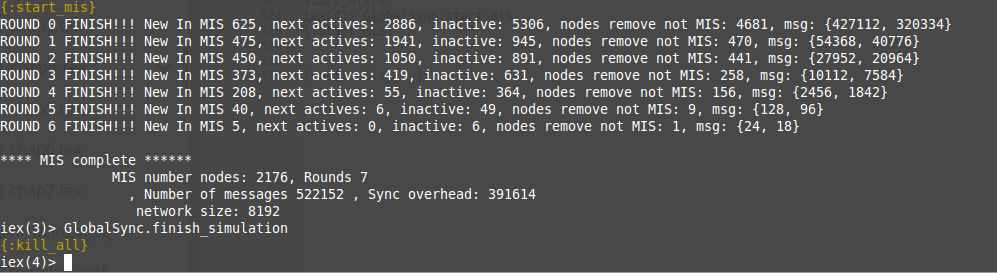
\includegraphics[width=0.9 \linewidth, height=5cm]{g_mis_run.png} 
\caption{Output of the execution of \textit{MIS} algorithm with global synchronizer}
\label{fig:gmis_run}
\end{figure}

To run algorithm using Alpha or Beta synchronizer the steps are similar. For these synchronizers, three modules should be compiled before running the algorithm, the module for the controller, \textbf{MIS} algorithm and synchronizer. The particular case is Beta because the rooted spanning tree should be constructed before running the algorithm. This is done calling the function \textbf{spanning\_tree}. The steps to execute the algorithm with Alpha and Beta are shown in \ref{code:alpha_exe} and \ref{code:beta_exe} respectively.



\begin{lstlisting}[style=terminal,caption= Example of compiling and executing the algorithm with Alpha, label = code:alpha_exe]

marcos@mtileriaPC ~/simulator/lib/alpha \$ iex
iex(1)> c "a_Controller.ex"
[A_controller]
iex(2)> c "a_mis.ex"     
[MIS]
iex(2)> c "Alpha.ex"     
[Alpha]
iex(3)> A_controller.start_nodes(8192)
:ok
iex(4)> A_controller.start_mis        
start_mis/0    
{:start_mis}
\end{lstlisting}

\begin{lstlisting}[style=terminal,caption= Example of compiling and executing the algorithm with Beta, label = code:beta_exe]

marcos@mtileriaPC ~/rhul/tesis/lib/beta \$ iex
iex(1)> c "b_Controller.ex"
[B_controller]
iex(2)> c "b_mis.ex"     
[MIS]
iex(2)> c "Beta.ex"     
[Beta]
iex(3)> B_controller.start_nodes(8192)
:ok
iex(4)> B_controller.start_mis        
start_mis/0    
{:start_mis}

\end{lstlisting}

